\documentclass{article}
\input{preamble.tex}

% Title
\title{12.3 The Pigeonhole Principle Revisited}
\author{Benjamin Basseri}


\begin{document}

\maketitle

\begin{problem}
Prove that if six integers are chosen at random, then at least two of them will have the same remainder when divided by 5.
\end{problem}

\textbf{Use the pigeonhole principle}. Let $A$ be any set of 6 integers, and $f$ be the function that maps an integer to its remainder after division by 5:
$$f: A \to \{0, 1, 2, 3, 4\}$$

$|A| = 6$ and the codomain is size 5. Since the domain is larger, $f$ cannot be injective which means there are at least 2 integers in $A$ with the same value mod 5

\begin{problem}
Prove that if $a$ is a natural number, then there exist two unequal natural numbers $k$ and $\ell$ for which $a^k - a^\ell$ is divisible by 10.
\end{problem}

The number $a^k - a^\ell$ will be divisible by 10 when $a^k$ and $a^\ell$ have the same value mod 10. There are 10 possible values modulo 10, that is 0 through 9. Consider possible values for $k$ and $\ell$ between 1 and 12 (so there are more than 10 choices), and let $f(n) = a^n \pmod{10}$. Then
$$f: [1, 12] \to [0, 9]$$
So $f$'s domain is strictly larger than its codomain. By the pigeonhole principle there are at least two distinct values $k, \ell \in [1, 12]$ such that $a^k \equiv a^\ell \pmod{10}$, which means their difference is divisble by 10.

\begin{problem}
Prove that for any six integers, 9 divides the sum or difference of two of them.
\end{problem}

We'll want to set this in the pigeonhole principle but also let's note that the difference of two numbers is divisible by 9 when the two numbers have the same value modulo 9. For their sum to be divisible by 9, their remainders must sum to 9.

If two of the six integers have the same value mod 9 then their difference is divisible by 9. If not, then it must be all six integers have different values mod 9, with 3 values unaccounted for. But since we have covered 6 of the 9 possible values mod 9, it must be that two of them are complements of each other (their remainders mod 9 sum to 9) because we have more than half the possibilities. Thus their sum will by divisible by 9.

But to more directly apply the pigeonhole principle, we can form a codomain that packages together those complements mod 9:
$$B = \{\{0\}, \{1, 8\}, \{2, 7\}, \{3, 6\}, \{4, 5\}\}$$

Now we can simply define $f(n) = \{n \pmod{9}, 9 - n \pmod{9}\}$. So $f$ maps an integer to which of those sets contains its value mod 9. Our domain is size 6 and the codomain 5, so this guarantees that there exists a pair of inputs $n, m$ mapping to the same output. If that output is $\{0\}$ then $n, m$ are both equivalent to 0 mod 9; their sum and difference will both be divisible by 9. Otherwise, the output is one of the sets containing two elements, e.g. $\{1, 8\}$. If $n, m$ have the same value mod 9 then their difference is divisble by 9. Otherwise, $n$ and $m$ have complementary values mod 9 (e.g. $n \pmod{9} = 1 \pmod{9}, m \pmod{n} = 8 \pmod{9})$ so their sum is divisble by 9.

\begin{problem}
Consider a square whose side-length is one unit. Select any five points from inside this square. Prove that at least two of these points are within $\sqrt{2}/2$ units of each other.
\end{problem}

If we subdivide the square into 4 subsquares $a, b, c, d$ each with side-length $1/2$ then their diagonals are $\sqrt{2}/2$. Then any two points in this square (including boundary) are at most $\sqrt{2}/2$ away from each other. Let $A$ be the set of 5 points and $B$ be the set of subsquares $\{a, b, c, d\}$. If we map a point to the subsquare containing it we have a function from $A$ to $B$ which must have two points mapping into the same subsquare, and therefore cannot be more than $\sqrt{2}/2$ apart.

Note: points on the boundary are technically in two subsquares, but we can then make a short proof by contradiction: suppose all 5 points are more than $\sqrt{2}/2$ apart and a point exists on the boundary of two subsquares. Then the point on the boundary `blocks out' both those subsquares; no other point can be in them or we'll violate the assumption they are at least $\sqrt{2}/2$ apart. Therefore all 4 points have to be in the remaining 2 subsquares. But here again by PHP this means there must be two points within $\sqrt{2}/2$.
\begin{center}

  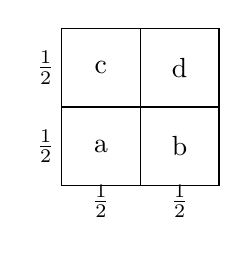
\begin{tikzpicture}
    % Draw the outer square
    \draw (0,0) rectangle (2,2);

    % Draw the inner subsquares
    \draw (1,0) -- (1,2);
    \draw (0,1) -- (2,1);

    % Label the side lengths
    \node at (0.5, -0.2) {$\frac{1}{2}$};
    \node at (1.5, -0.2) {$\frac{1}{2}$};
    \node at (-0.2, 0.5) {$\frac{1}{2}$};
    \node at (-0.2, 1.5) {$\frac{1}{2}$};

    % Label the subsquares
    \node at (0.5, 0.5) {a};
    \node at (1.5, 0.5) {b};
    \node at (0.5, 1.5) {c};
    \node at (1.5, 1.5) {d};
  \end{tikzpicture}
\end{center}

\begin{problem}
Prove that any set of seven distinct integers contains a pair of integers whose sum or difference is divisible by 10.
\end{problem}

Note that any pair of integers can form a difference or a sum; the difference is divisible by 10 when both integers are equivalent mod 10, and the sum is divisible by 10 when the integers' remainders are complements of each other (e.g. 1 and 9, 2 and 8).

So if two integers have the same remainder OR complementary remainders, then their sum or difference will be divisible by 10. Setting this into PHP, let $A$ be any set of 7 distinct integers, and let $B$ be
$$B = \{\{0\}, \{1, 9\}, \{2, 8\}, \{3, 7\}, \{4, 6\}, \{5\}\}$$

If we let $f$ be the function that maps $n$ to the set in $B$ containing its remainder, then since $|A| = 7, |B| = 6$, the function $f$ can't be injective and two integers in $A$ map to the same set in $B$. This means either their sum or their difference is divisible by 10.

\begin{problem}
Given a sphere $S$ a \textit{great circle} of $S$ is the intersection of $S$ with a plane through its center. Every great circle divides $S$ into two parts. A \textit{hemisphere} is the union of the great circle and one of these two parts. Prove that if five points are placed arbitrarily on $S$, then there is a hemisphere that contains four of them.
\end{problem}


Any two points on the sphere determines a great circle, which determines a hemisphere. So take two of the 5 points to determine two hemispheres. There are 3 points remaining, so one of the hemispheres contains at least 2 of them. This hemisphere then has at least 4 of the 5 points.

\begin{problem}
Prove or disprove: Any subset $X \subseteq \{1, 2, 3, \ldots, 2n\}$ with $|X| > n$ contains two (unequal) elements for which one divides the other.
\end{problem}

Constructive proof: we can write any $x \in X$ as $2^p q$ where $q$ is the largest odd integer dividing $x$. If we map $X$ elements to the largest odd number that divides it, the codomain would be $Y = \{1, 3, 5, \ldots, 2n - 1\}$ which has size $n$. Since $|X| > n$ the mapping to $Y$ can't be injective, meaning there are distinct $a, b \in X$ where $f(a) = f(b)$. This means:
$$a = 2^p q, \quad b = 2^r q$$

Since they're equal on $f$ they have the same odd divisor, and differ only in their power of 2. Since they're distinct either $a < b$ or $b < a$, WLOG suppose $a < b$ then $a = 2^p q$ and $b = 2^{p+k}q$ for some $k$. Then $a \mid b$.


\end{document}